\documentclass{standalone}
\usepackage{tikz}
\usetikzlibrary{patterns, positioning}


\begin{document}
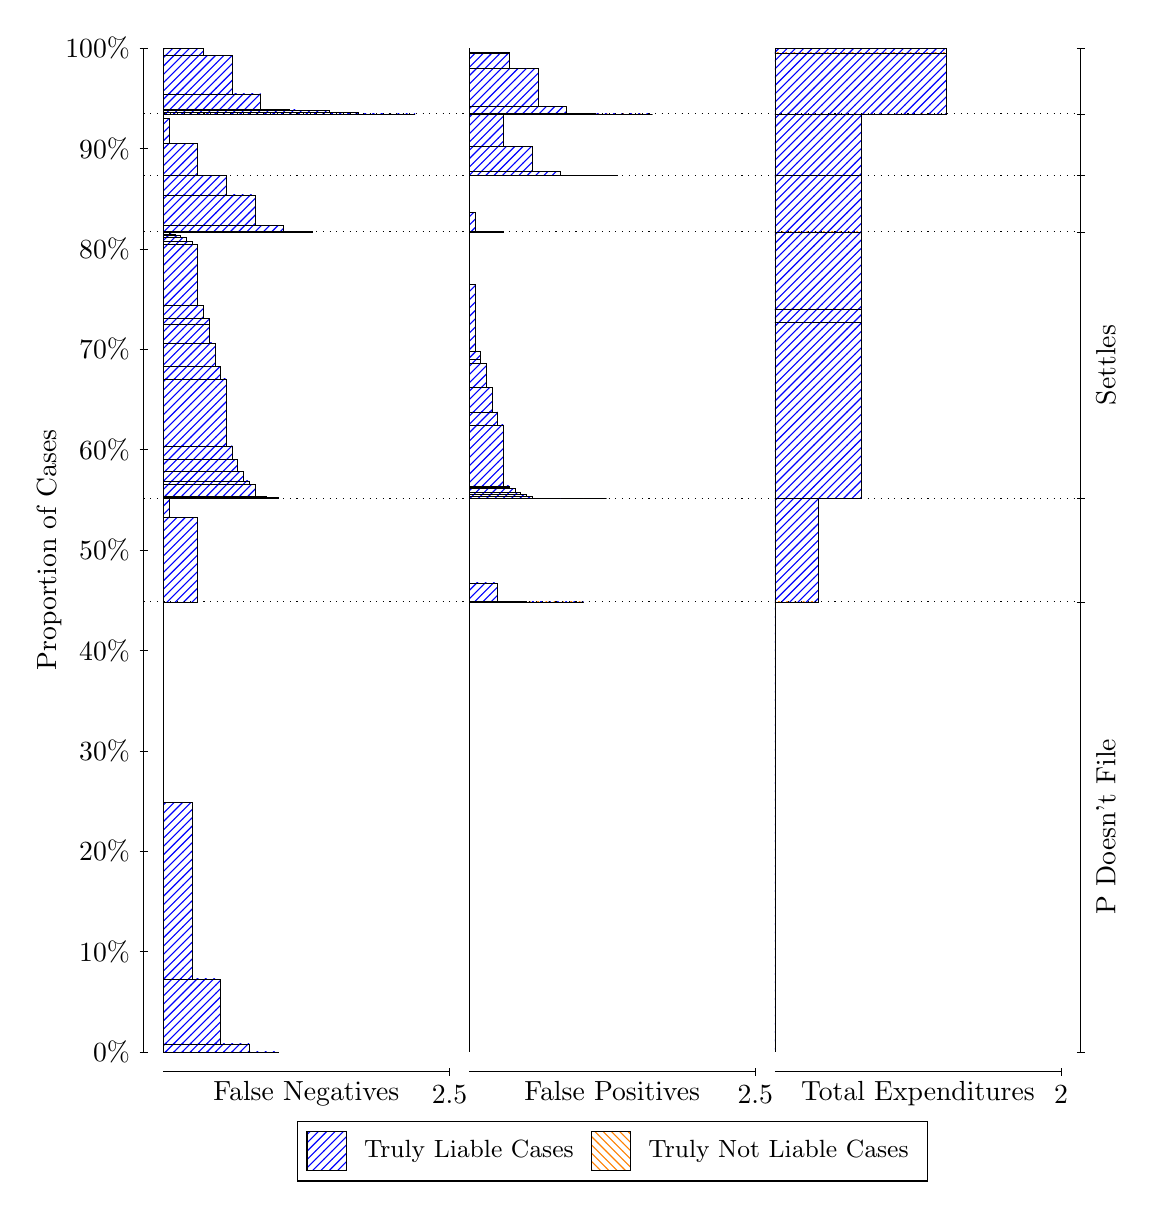
\begin{tikzpicture}
\draw[black, very thin] (1.5,1.75) -- (1.5,14.5);
\node[rotate=90, text=black, anchor=center] at (0.3, 8.125) {Proportion of Cases};
\draw[black, very thin] (1.45,1.75) -- (1.55,1.75);
\node[text=black, anchor=east] at (1.45, 1.75) {0\%};
\draw[black, very thin] (1.45,3.025) -- (1.55,3.025);
\node[text=black, anchor=east] at (1.45, 3.025) {10\%};
\draw[black, very thin] (1.45,4.3) -- (1.55,4.3);
\node[text=black, anchor=east] at (1.45, 4.3) {20\%};
\draw[black, very thin] (1.45,5.575) -- (1.55,5.575);
\node[text=black, anchor=east] at (1.45, 5.575) {30\%};
\draw[black, very thin] (1.45,6.85) -- (1.55,6.85);
\node[text=black, anchor=east] at (1.45, 6.85) {40\%};
\draw[black, very thin] (1.45,8.125) -- (1.55,8.125);
\node[text=black, anchor=east] at (1.45, 8.125) {50\%};
\draw[black, very thin] (1.45,9.4) -- (1.55,9.4);
\node[text=black, anchor=east] at (1.45, 9.4) {60\%};
\draw[black, very thin] (1.45,10.675) -- (1.55,10.675);
\node[text=black, anchor=east] at (1.45, 10.675) {70\%};
\draw[black, very thin] (1.45,11.95) -- (1.55,11.95);
\node[text=black, anchor=east] at (1.45, 11.95) {80\%};
\draw[black, very thin] (1.45,13.225) -- (1.55,13.225);
\node[text=black, anchor=east] at (1.45, 13.225) {90\%};
\draw[black, very thin] (1.45,14.5) -- (1.55,14.5);
\node[text=black, anchor=east] at (1.45, 14.5) {100\%};

\draw[black, very thin] (13.4,1.75) -- (13.4,14.5);
\draw[black, very thin] (13.35,1.75) -- (13.45,1.75);
\node[anchor=west] at (13.35, 1.75) {};
\draw[black, very thin] (13.35,7.4672) -- (13.45,7.4672);
\node[anchor=west] at (13.35, 7.4672) {};
\draw[black, very thin] (13.35,8.7826) -- (13.45,8.7826);
\node[anchor=west] at (13.35, 8.7826) {};
\draw[black, very thin] (13.35,12.166) -- (13.45,12.166);
\node[anchor=west] at (13.35, 12.166) {};
\draw[black, very thin] (13.35,12.881) -- (13.45,12.881);
\node[anchor=west] at (13.35, 12.881) {};
\draw[black, very thin] (13.35,13.664) -- (13.45,13.664);
\node[anchor=west] at (13.35, 13.664) {};
\draw[black, very thin] (13.35,14.5) -- (13.45,14.5);
\node[anchor=west] at (13.35, 14.5) {};

\draw[black, very thin, pattern color=blue, pattern=north east lines] (1.75,1.75) rectangle (3.2033,1.751);
\draw[black, very thin, pattern color=blue, pattern=north east lines] (1.75,1.751) rectangle (2.84,1.8517);
\draw[black, very thin, pattern color=blue, pattern=north east lines] (1.75,1.8517) rectangle (2.4767,2.6781);
\draw[black, very thin, pattern color=blue, pattern=north east lines] (1.75,2.6781) rectangle (2.1133,4.9203);
\draw[black, very thin, pattern color=orange, pattern=north west lines] (1.75,4.9203) rectangle (1.75,4.9203);
\draw[black, very thin, pattern color=blue, pattern=north east lines] (1.75,4.9203) rectangle (1.75,7.4672);
\draw[black, very thin, pattern color=blue, pattern=north east lines] (1.75,7.4672) rectangle (2.186,8.5436);
\draw[black, very thin, pattern color=blue, pattern=north east lines] (1.75,8.5436) rectangle (1.8227,8.776);
\draw[black, very thin, pattern color=orange, pattern=north west lines] (1.75,8.776) rectangle (1.75,8.776);
\draw[black, very thin, pattern color=blue, pattern=north east lines] (1.75,8.776) rectangle (1.75,8.7826);
\draw[black, very thin, pattern color=blue, pattern=north east lines] (1.75,8.7826) rectangle (3.2033,8.7888);
\draw[black, very thin, pattern color=blue, pattern=north east lines] (1.75,8.7888) rectangle (3.058,8.8031);
\draw[black, very thin, pattern color=blue, pattern=north east lines] (1.75,8.8031) rectangle (2.9127,8.9579);
\draw[black, very thin, pattern color=blue, pattern=north east lines] (1.75,8.9579) rectangle (2.84,9.0023);
\draw[black, very thin, pattern color=blue, pattern=north east lines] (1.75,9.0023) rectangle (2.7673,9.119);
\draw[black, very thin, pattern color=blue, pattern=north east lines] (1.75,9.119) rectangle (2.6947,9.2804);
\draw[black, very thin, pattern color=blue, pattern=north east lines] (1.75,9.2804) rectangle (2.622,9.4473);
\draw[black, very thin, pattern color=blue, pattern=north east lines] (1.75,9.4473) rectangle (2.5493,10.297);
\draw[black, very thin, pattern color=blue, pattern=north east lines] (1.75,10.297) rectangle (2.4767,10.456);
\draw[black, very thin, pattern color=blue, pattern=north east lines] (1.75,10.456) rectangle (2.404,10.756);
\draw[black, very thin, pattern color=blue, pattern=north east lines] (1.75,10.756) rectangle (2.3313,10.993);
\draw[black, very thin, pattern color=blue, pattern=north east lines] (1.75,10.993) rectangle (2.3313,11.07);
\draw[black, very thin, pattern color=blue, pattern=north east lines] (1.75,11.07) rectangle (2.2587,11.234);
\draw[black, very thin, pattern color=blue, pattern=north east lines] (1.75,11.234) rectangle (2.186,12.009);
\draw[black, very thin, pattern color=blue, pattern=north east lines] (1.75,12.009) rectangle (2.1133,12.045);
\draw[black, very thin, pattern color=blue, pattern=north east lines] (1.75,12.045) rectangle (2.0407,12.093);
\draw[black, very thin, pattern color=blue, pattern=north east lines] (1.75,12.093) rectangle (1.968,12.102);
\draw[black, very thin, pattern color=blue, pattern=north east lines] (1.75,12.102) rectangle (1.968,12.118);
\draw[black, very thin, pattern color=blue, pattern=north east lines] (1.75,12.118) rectangle (1.8953,12.139);
\draw[black, very thin, pattern color=blue, pattern=north east lines] (1.75,12.139) rectangle (1.8227,12.165);
\draw[black, very thin, pattern color=orange, pattern=north west lines] (1.75,12.165) rectangle (1.75,12.165);
\draw[black, very thin, pattern color=blue, pattern=north east lines] (1.75,12.165) rectangle (1.75,12.166);
\draw[black, very thin, pattern color=blue, pattern=north east lines] (1.75,12.166) rectangle (3.6393,12.174);
\draw[black, very thin, pattern color=blue, pattern=north east lines] (1.75,12.174) rectangle (3.276,12.251);
\draw[black, very thin, pattern color=blue, pattern=north east lines] (1.75,12.251) rectangle (2.9127,12.634);
\draw[black, very thin, pattern color=blue, pattern=north east lines] (1.75,12.634) rectangle (2.5493,12.878);
\draw[black, very thin, pattern color=blue, pattern=north east lines] (1.75,12.878) rectangle (2.186,12.881);
\draw[black, very thin, pattern color=orange, pattern=north west lines] (1.75,12.881) rectangle (1.75,12.881);
\draw[black, very thin, pattern color=blue, pattern=north east lines] (1.75,12.881) rectangle (2.186,13.29);
\draw[black, very thin, pattern color=blue, pattern=north east lines] (1.75,13.29) rectangle (1.8227,13.606);
\draw[black, very thin, pattern color=orange, pattern=north west lines] (1.75,13.606) rectangle (1.75,13.606);
\draw[black, very thin, pattern color=blue, pattern=north east lines] (1.75,13.606) rectangle (1.75,13.664);
\draw[black, very thin, pattern color=blue, pattern=north east lines] (1.75,13.664) rectangle (4.9473,13.664);
\draw[black, very thin, pattern color=blue, pattern=north east lines] (1.75,13.664) rectangle (4.584,13.664);
\draw[black, very thin, pattern color=blue, pattern=north east lines] (1.75,13.664) rectangle (4.2207,13.678);
\draw[black, very thin, pattern color=blue, pattern=north east lines] (1.75,13.678) rectangle (3.8573,13.712);
\draw[black, very thin, pattern color=blue, pattern=north east lines] (1.75,13.712) rectangle (3.712,13.712);
\draw[black, very thin, pattern color=blue, pattern=north east lines] (1.75,13.712) rectangle (3.494,13.714);
\draw[black, very thin, pattern color=blue, pattern=north east lines] (1.75,13.714) rectangle (3.3487,13.722);
\draw[black, very thin, pattern color=blue, pattern=north east lines] (1.75,13.722) rectangle (3.1307,13.722);
\draw[black, very thin, pattern color=blue, pattern=north east lines] (1.75,13.722) rectangle (2.9853,13.918);
\draw[black, very thin, pattern color=blue, pattern=north east lines] (1.75,13.918) rectangle (2.7673,13.918);
\draw[black, very thin, pattern color=blue, pattern=north east lines] (1.75,13.918) rectangle (2.622,14.41);
\draw[black, very thin, pattern color=blue, pattern=north east lines] (1.75,14.41) rectangle (2.2587,14.498);
\draw[black, very thin, pattern color=blue, pattern=north east lines] (1.75,14.498) rectangle (1.8953,14.5);
\draw[black, very thin, pattern color=orange, pattern=north west lines] (1.75,14.5) rectangle (1.75,14.5);
\draw[black, very thin, pattern color=blue, pattern=north east lines] (1.75,14.5) rectangle (1.75,14.5);
\draw[black, very thin, pattern color=orange, pattern=north west lines] (5.6333,1.75) rectangle (5.6333,1.75);
\draw[black, very thin, pattern color=blue, pattern=north east lines] (5.6333,1.75) rectangle (5.6333,7.4672);
\draw[black, very thin, pattern color=orange, pattern=north west lines] (5.6333,7.4672) rectangle (7.0867,7.4672);
\draw[black, very thin, pattern color=blue, pattern=north east lines] (5.6333,7.4672) rectangle (7.0867,7.4672);
\draw[black, very thin, pattern color=blue, pattern=north east lines] (5.6333,7.4672) rectangle (6.7233,7.4672);
\draw[black, very thin, pattern color=blue, pattern=north east lines] (5.6333,7.4672) rectangle (6.36,7.4738);
\draw[black, very thin, pattern color=blue, pattern=north east lines] (5.6333,7.4738) rectangle (5.9967,7.7063);
\draw[black, very thin, pattern color=blue, pattern=north east lines] (5.6333,7.7063) rectangle (5.6333,8.7826);
\draw[black, very thin, pattern color=orange, pattern=north west lines] (5.6333,8.7826) rectangle (7.3773,8.7826);
\draw[black, very thin, pattern color=blue, pattern=north east lines] (5.6333,8.7826) rectangle (7.3773,8.7826);
\draw[black, very thin, pattern color=orange, pattern=north west lines] (5.6333,8.7826) rectangle (7.232,8.7826);
\draw[black, very thin, pattern color=blue, pattern=north east lines] (5.6333,8.7826) rectangle (7.232,8.7826);
\draw[black, very thin, pattern color=orange, pattern=north west lines] (5.6333,8.7826) rectangle (7.0867,8.7826);
\draw[black, very thin, pattern color=blue, pattern=north east lines] (5.6333,8.7826) rectangle (7.0867,8.7826);
\draw[black, very thin, pattern color=blue, pattern=north east lines] (5.6333,8.7826) rectangle (7.014,8.7826);
\draw[black, very thin, pattern color=orange, pattern=north west lines] (5.6333,8.7826) rectangle (6.9413,8.7826);
\draw[black, very thin, pattern color=blue, pattern=north east lines] (5.6333,8.7826) rectangle (6.9413,8.7826);
\draw[black, very thin, pattern color=blue, pattern=north east lines] (5.6333,8.7826) rectangle (6.8687,8.7826);
\draw[black, very thin, pattern color=orange, pattern=north west lines] (5.6333,8.7826) rectangle (6.796,8.7826);
\draw[black, very thin, pattern color=blue, pattern=north east lines] (5.6333,8.7826) rectangle (6.796,8.7826);
\draw[black, very thin, pattern color=blue, pattern=north east lines] (5.6333,8.7826) rectangle (6.7233,8.7827);
\draw[black, very thin, pattern color=orange, pattern=north west lines] (5.6333,8.7827) rectangle (6.6507,8.7827);
\draw[black, very thin, pattern color=blue, pattern=north east lines] (5.6333,8.7827) rectangle (6.6507,8.7827);
\draw[black, very thin, pattern color=blue, pattern=north east lines] (5.6333,8.7827) rectangle (6.578,8.7828);
\draw[black, very thin, pattern color=blue, pattern=north east lines] (5.6333,8.7828) rectangle (6.5053,8.7829);
\draw[black, very thin, pattern color=orange, pattern=north west lines] (5.6333,8.7829) rectangle (6.5053,8.7829);
\draw[black, very thin, pattern color=blue, pattern=north east lines] (5.6333,8.7829) rectangle (6.5053,8.783);
\draw[black, very thin, pattern color=blue, pattern=north east lines] (5.6333,8.783) rectangle (6.4327,8.8099);
\draw[black, very thin, pattern color=blue, pattern=north east lines] (5.6333,8.8099) rectangle (6.36,8.8305);
\draw[black, very thin, pattern color=blue, pattern=north east lines] (5.6333,8.8305) rectangle (6.2873,8.8555);
\draw[black, very thin, pattern color=blue, pattern=north east lines] (5.6333,8.8555) rectangle (6.2147,8.903);
\draw[black, very thin, pattern color=blue, pattern=north east lines] (5.6333,8.903) rectangle (6.142,8.9162);
\draw[black, very thin, pattern color=blue, pattern=north east lines] (5.6333,8.9162) rectangle (6.142,8.9394);
\draw[black, very thin, pattern color=blue, pattern=north east lines] (5.6333,8.9394) rectangle (6.0693,9.7148);
\draw[black, very thin, pattern color=blue, pattern=north east lines] (5.6333,9.7148) rectangle (5.9967,9.878);
\draw[black, very thin, pattern color=blue, pattern=north east lines] (5.6333,9.878) rectangle (5.924,10.192);
\draw[black, very thin, pattern color=blue, pattern=north east lines] (5.6333,10.192) rectangle (5.8513,10.492);
\draw[black, very thin, pattern color=blue, pattern=north east lines] (5.6333,10.492) rectangle (5.7787,10.55);
\draw[black, very thin, pattern color=blue, pattern=north east lines] (5.6333,10.55) rectangle (5.7787,10.651);
\draw[black, very thin, pattern color=blue, pattern=north east lines] (5.6333,10.651) rectangle (5.706,11.501);
\draw[black, very thin, pattern color=blue, pattern=north east lines] (5.6333,11.501) rectangle (5.6333,12.166);
\draw[black, very thin, pattern color=orange, pattern=north west lines] (5.6333,12.166) rectangle (6.0693,12.166);
\draw[black, very thin, pattern color=blue, pattern=north east lines] (5.6333,12.166) rectangle (6.0693,12.169);
\draw[black, very thin, pattern color=blue, pattern=north east lines] (5.6333,12.169) rectangle (5.706,12.413);
\draw[black, very thin, pattern color=blue, pattern=north east lines] (5.6333,12.413) rectangle (5.6333,12.881);
\draw[black, very thin, pattern color=orange, pattern=north west lines] (5.6333,12.881) rectangle (7.5227,12.881);
\draw[black, very thin, pattern color=blue, pattern=north east lines] (5.6333,12.881) rectangle (7.5227,12.881);
\draw[black, very thin, pattern color=blue, pattern=north east lines] (5.6333,12.881) rectangle (7.1593,12.882);
\draw[black, very thin, pattern color=blue, pattern=north east lines] (5.6333,12.882) rectangle (6.796,12.938);
\draw[black, very thin, pattern color=blue, pattern=north east lines] (5.6333,12.938) rectangle (6.4327,13.255);
\draw[black, very thin, pattern color=blue, pattern=north east lines] (5.6333,13.255) rectangle (6.0693,13.664);
\draw[black, very thin, pattern color=orange, pattern=north west lines] (5.6333,13.664) rectangle (7.9587,13.664);
\draw[black, very thin, pattern color=blue, pattern=north east lines] (5.6333,13.664) rectangle (7.9587,13.664);
\draw[black, very thin, pattern color=orange, pattern=north west lines] (5.6333,13.664) rectangle (7.5953,13.664);
\draw[black, very thin, pattern color=blue, pattern=north east lines] (5.6333,13.664) rectangle (7.5953,13.664);
\draw[black, very thin, pattern color=orange, pattern=north west lines] (5.6333,13.664) rectangle (7.232,13.664);
\draw[black, very thin, pattern color=blue, pattern=north east lines] (5.6333,13.664) rectangle (7.232,13.666);
\draw[black, very thin, pattern color=blue, pattern=north east lines] (5.6333,13.666) rectangle (6.8687,13.754);
\draw[black, very thin, pattern color=orange, pattern=north west lines] (5.6333,13.754) rectangle (6.8687,13.754);
\draw[black, very thin, pattern color=blue, pattern=north east lines] (5.6333,13.754) rectangle (6.8687,13.754);
\draw[black, very thin, pattern color=blue, pattern=north east lines] (5.6333,13.754) rectangle (6.5053,14.245);
\draw[black, very thin, pattern color=blue, pattern=north east lines] (5.6333,14.245) rectangle (6.5053,14.246);
\draw[black, very thin, pattern color=orange, pattern=north west lines] (5.6333,14.246) rectangle (6.36,14.246);
\draw[black, very thin, pattern color=blue, pattern=north east lines] (5.6333,14.246) rectangle (6.36,14.246);
\draw[black, very thin, pattern color=blue, pattern=north east lines] (5.6333,14.246) rectangle (6.142,14.432);
\draw[black, very thin, pattern color=blue, pattern=north east lines] (5.6333,14.432) rectangle (6.142,14.441);
\draw[black, very thin, pattern color=orange, pattern=north west lines] (5.6333,14.441) rectangle (5.9967,14.441);
\draw[black, very thin, pattern color=blue, pattern=north east lines] (5.6333,14.441) rectangle (5.9967,14.441);
\draw[black, very thin, pattern color=blue, pattern=north east lines] (5.6333,14.441) rectangle (5.7787,14.447);
\draw[black, very thin, pattern color=blue, pattern=north east lines] (5.6333,14.447) rectangle (5.7787,14.449);
\draw[black, very thin, pattern color=orange, pattern=north west lines] (5.6333,14.449) rectangle (5.6333,14.449);
\draw[black, very thin, pattern color=blue, pattern=north east lines] (5.6333,14.449) rectangle (5.6333,14.5);
\draw[black, very thin, pattern color=orange, pattern=north west lines] (9.5167,1.75) rectangle (9.5167,1.75);
\draw[black, very thin, pattern color=blue, pattern=north east lines] (9.5167,1.75) rectangle (9.5167,7.4672);
\draw[black, very thin, pattern color=orange, pattern=north west lines] (9.5167,7.4672) rectangle (10.062,7.4672);
\draw[black, very thin, pattern color=blue, pattern=north east lines] (9.5167,7.4672) rectangle (10.062,8.7826);
\draw[black, very thin, pattern color=orange, pattern=north west lines] (9.5167,8.7826) rectangle (10.607,8.7826);
\draw[black, very thin, pattern color=blue, pattern=north east lines] (9.5167,8.7826) rectangle (10.607,11.011);
\draw[black, very thin, pattern color=orange, pattern=north west lines] (9.5167,11.011) rectangle (10.607,11.011);
\draw[black, very thin, pattern color=blue, pattern=north east lines] (9.5167,11.011) rectangle (10.607,11.186);
\draw[black, very thin, pattern color=orange, pattern=north west lines] (9.5167,11.186) rectangle (10.607,11.186);
\draw[black, very thin, pattern color=blue, pattern=north east lines] (9.5167,11.186) rectangle (10.607,12.166);
\draw[black, very thin, pattern color=orange, pattern=north west lines] (9.5167,12.166) rectangle (10.607,12.166);
\draw[black, very thin, pattern color=blue, pattern=north east lines] (9.5167,12.166) rectangle (10.607,12.881);
\draw[black, very thin, pattern color=orange, pattern=north west lines] (9.5167,12.881) rectangle (10.607,12.881);
\draw[black, very thin, pattern color=blue, pattern=north east lines] (9.5167,12.881) rectangle (10.607,13.664);
\draw[black, very thin, pattern color=orange, pattern=north west lines] (9.5167,13.664) rectangle (11.697,13.664);
\draw[black, very thin, pattern color=blue, pattern=north east lines] (9.5167,13.664) rectangle (11.697,14.438);
\draw[black, very thin, pattern color=orange, pattern=north west lines] (9.5167,14.438) rectangle (11.697,14.438);
\draw[black, very thin, pattern color=blue, pattern=north east lines] (9.5167,14.438) rectangle (11.697,14.5);
\draw[black, dotted] (1.5,7.4672) -- (13.4,7.4672);
\draw[black, dotted] (1.5,8.7826) -- (13.4,8.7826);
\draw[black, dotted] (1.5,12.166) -- (13.4,12.166);
\draw[black, dotted] (1.5,12.881) -- (13.4,12.881);
\draw[black, dotted] (1.5,13.664) -- (13.4,13.664);
\draw[black, very thin] (1.75,1.5) -- (5.3833,1.5);
\node[text=black, anchor=north] at (3.5667, 1.5) {False Negatives};
\draw[black, very thin] (5.3833,1.45) -- (5.3833,1.55);
\node[text=black, anchor=north] at (5.3833, 1.45) {2.5};

\draw[black, very thin] (5.6333,1.5) -- (9.2667,1.5);
\node[text=black, anchor=north] at (7.45, 1.5) {False Positives};
\draw[black, very thin] (9.2667,1.45) -- (9.2667,1.55);
\node[text=black, anchor=north] at (9.2667, 1.45) {2.5};

\draw[black, very thin] (9.5167,1.5) -- (13.15,1.5);
\node[text=black, anchor=north] at (11.333, 1.5) {Total Expenditures};
\draw[black, very thin] (13.15,1.45) -- (13.15,1.55);
\node[text=black, anchor=north] at (13.15, 1.45) {2};

\node[text=black, centered, rotate=90] at (13.72, 4.6086) {P Doesn't File};

\node[text=black, centered, rotate=90] at (13.72, 10.474) {Settles};




\draw (7.449999999999999,1.5) node[draw=none] (baseCoordinate) {};
\begin{scope}[align=center]
        \matrix[scale=0.5, draw=black, below=0.5cm of baseCoordinate, nodes={draw}, column sep=0.1cm]{
            \node[rectangle, draw, minimum width=0.5cm, minimum height=0.5cm, pattern color=blue, pattern=north east lines] {}; &
            \node[draw=none, font=\small, text=black] (B) {Truly Liable Cases}; &
            \node[rectangle, draw, minimum width=0.5cm, minimum height=0.5cm, pattern color=orange, pattern=north west lines] {}; &
            \node[draw=none, font=\small, text=black] (B) {Truly Not Liable Cases}; \\
            };
\end{scope}

\end{tikzpicture}
\end{document}